\section{Magnitude Conversion}

In this study we use two sets of data, i.e., historical and instrumental seismic catalogs. We use the historical catalog reported by \citep{Karimiparidari2013}, which is converted into $M_w$ magnitude. Fig.~\ref{fig:historical} shows the historical earthquakes (pre-1900) in northern Iran. The instrumental data has been reported mainly by the International Institute of Earthquake Engineering and Seismology of Iran \citep{IIEES}, and are reported in $M_L$ magnitude type. In this study we use the relationship that proposed by \citet{Karimiparidari2013}, to convert local magnitude into moment magnitude. 

\begin{figure} [H]
\centering
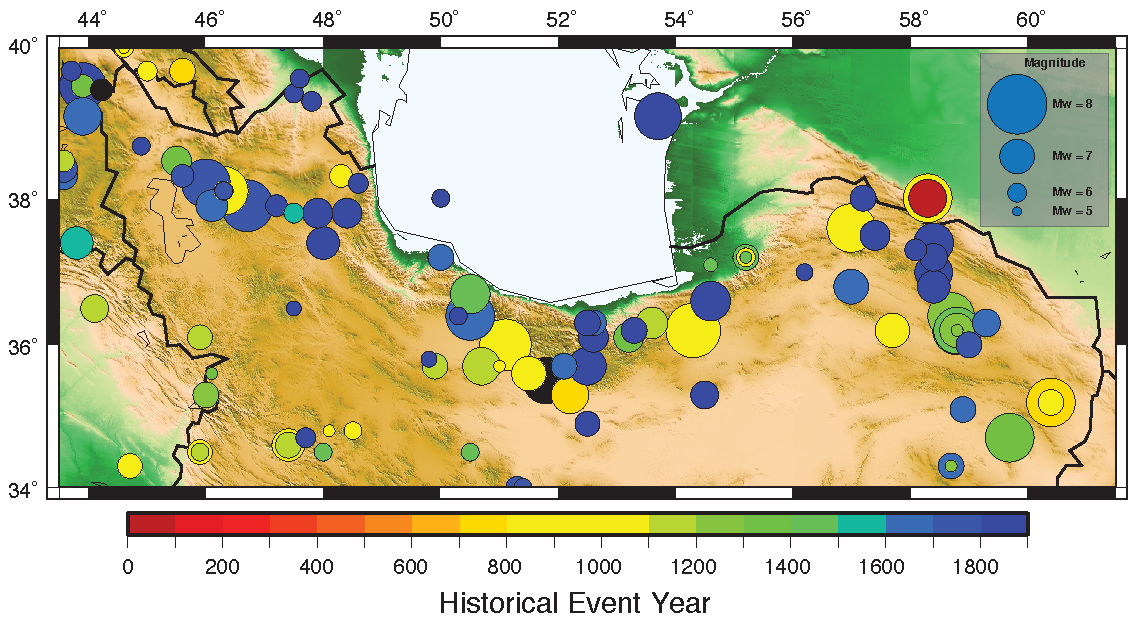
\includegraphics[scale=0.8]{figures/pdf/Figure2.pdf} 
\caption{Historical earthquakes of Iran (pre 1900). Different colors represent different year of occurrences and size of circles are proportional to the earthquake magnitude. }
\label{fig:historical}
\end{figure}
